\chapter{Methodology}
\label{ch:methodology}

This chapter presents a comprehensive methodology for adaptive detection of fileless and polymorphic malware through an integrated approach combining memory forensics, computer vision, and machine learning techniques. The proposed framework addresses the fundamental limitations of traditional signature-based detection systems by analyzing memory-resident patterns and employing advanced dimensional reduction techniques to enhance unknown malware identification capabilities.


\begin{figure}[!htbp]
    \centering
    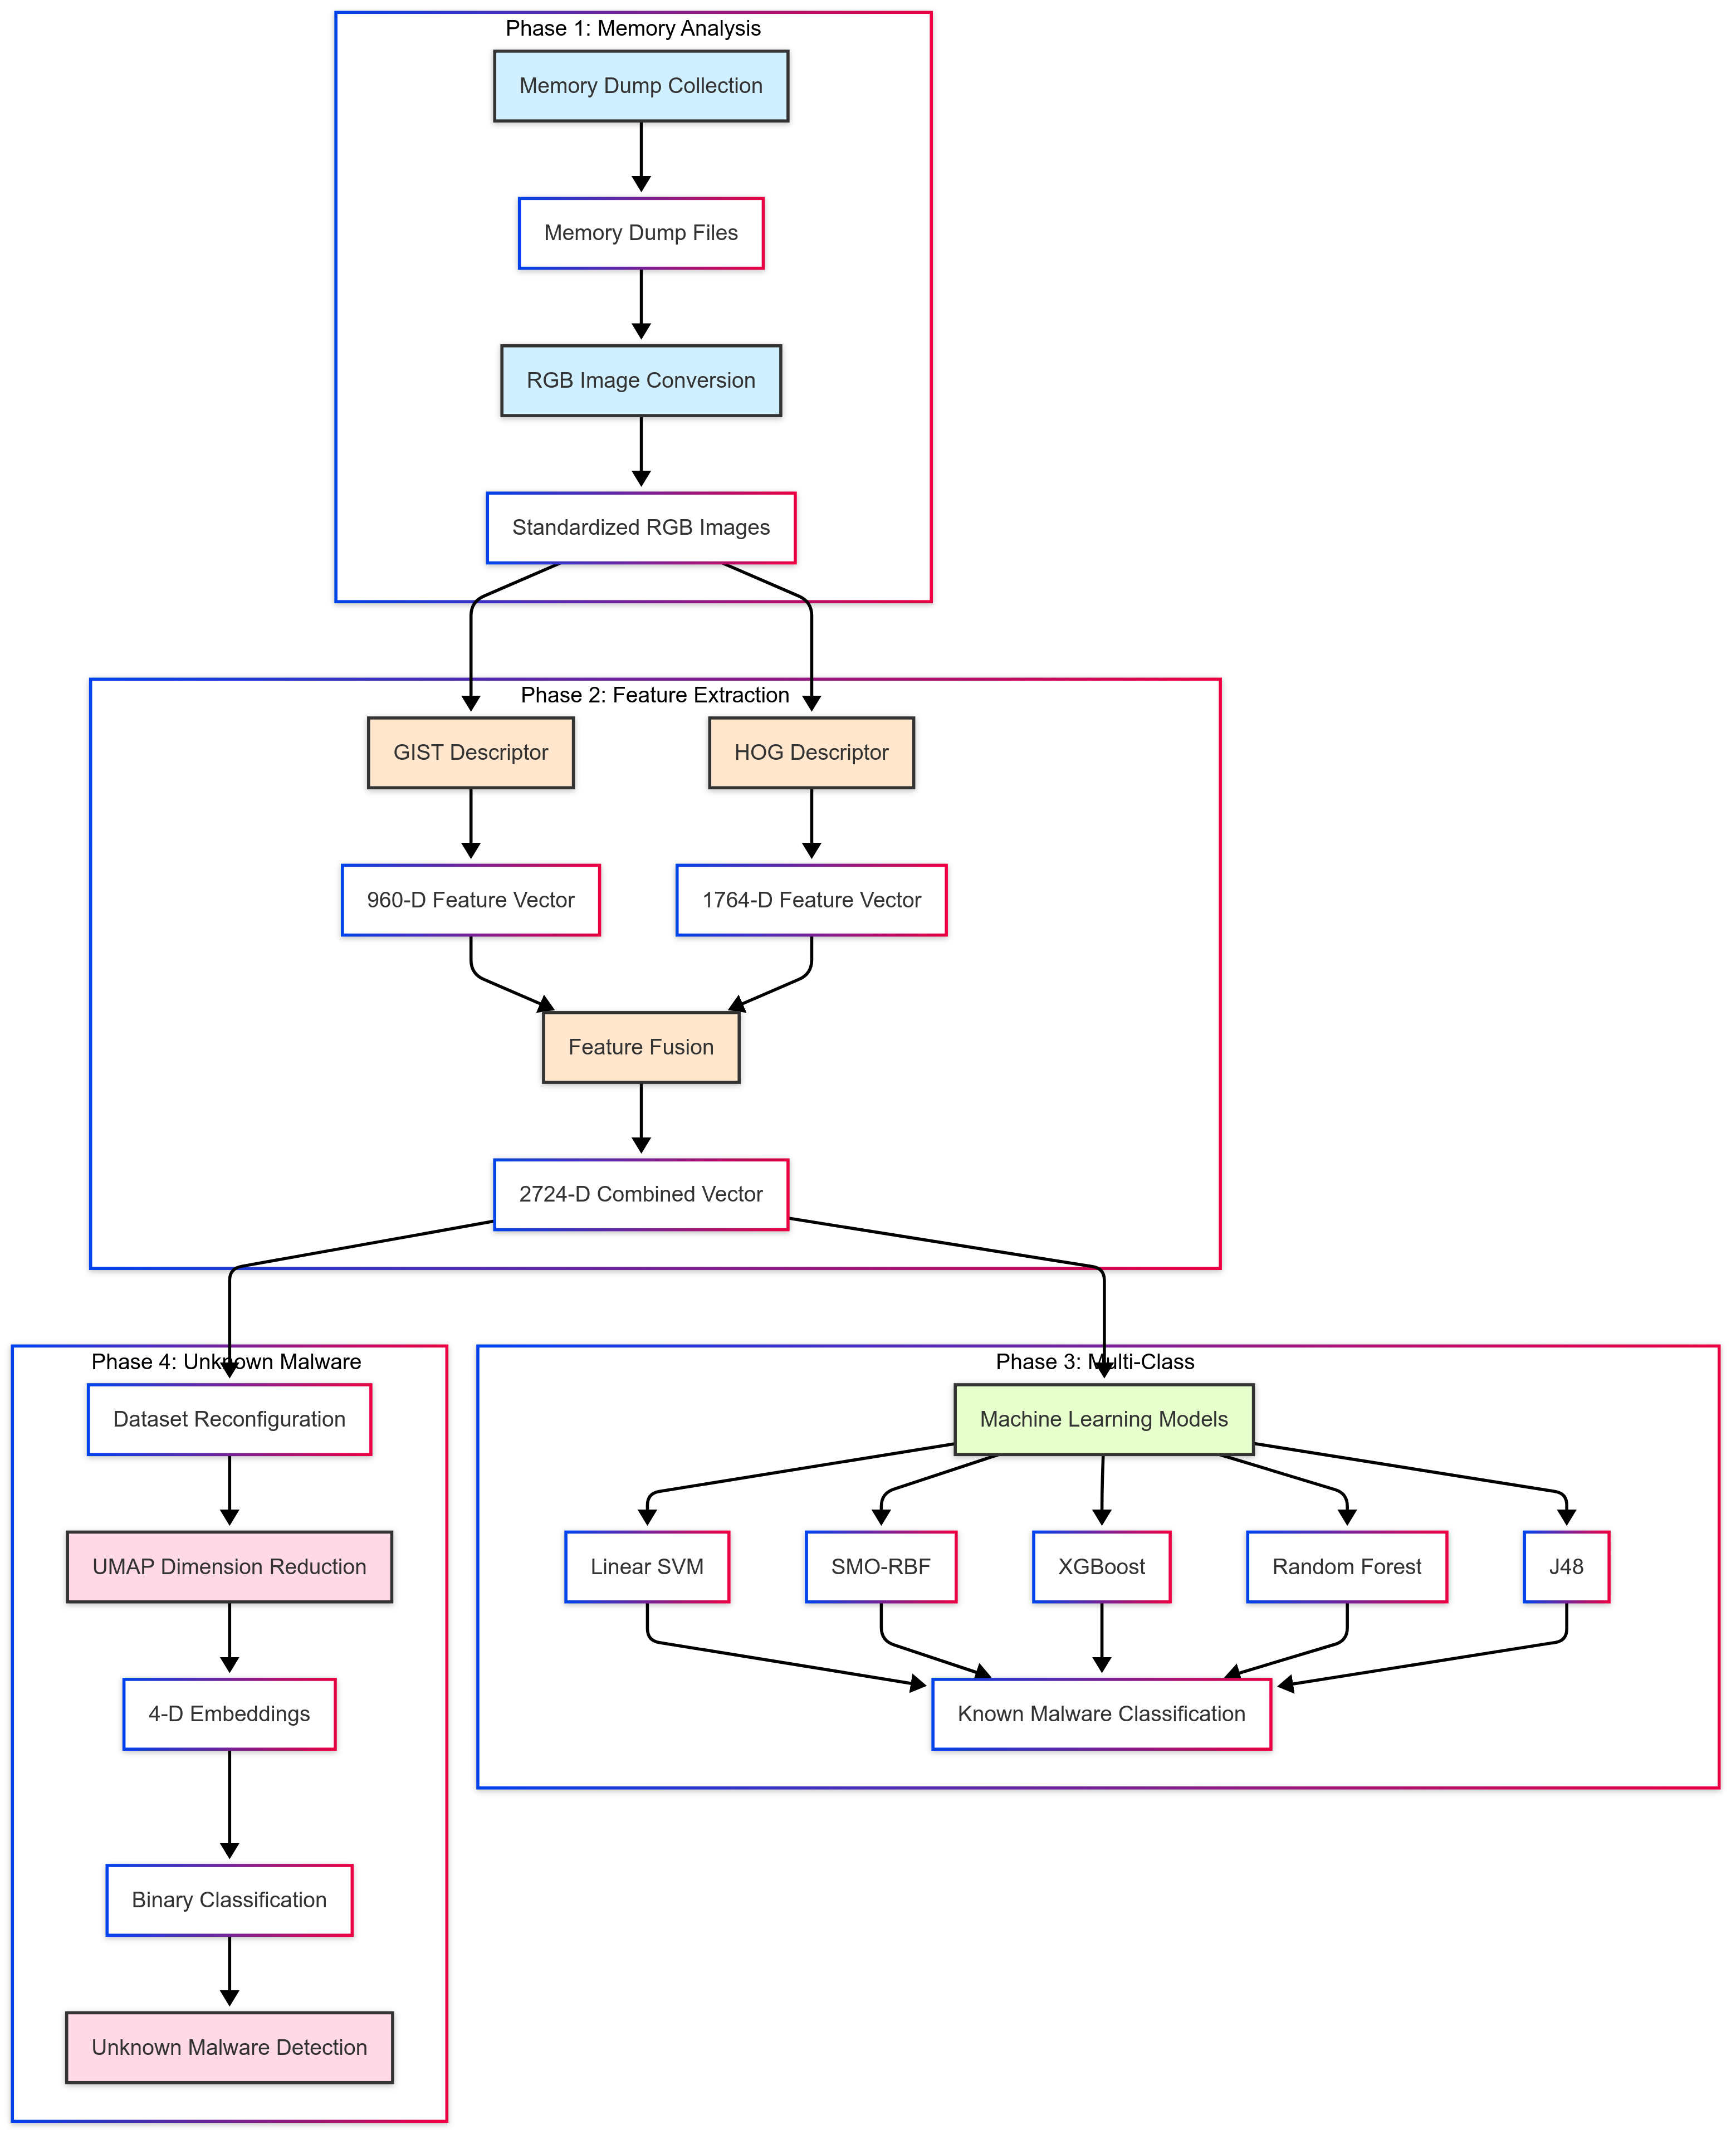
\includegraphics[width=0.9\textwidth]{figures/methodology.png}
    \caption{Comprehensive workflow of the proposed malware detection framework, showing the four main phases: Memory Analysis, Feature Extraction, Multi-Class Classification, and Unknown Malware Detection.}
    \label{fig:methodology-overview}
\end{figure}

\section{Overview of the Proposed Framework}
\label{sec:methodology-overview}

The methodology encompasses a multi-phase approach designed to capture, analyze, and classify malware behavior through memory-based analysis. Figure~\ref{fig:methodology-overview} illustrates the complete workflow of our proposed detection framework.

The proposed framework consists of four main phases:

\begin{enumerate}
    \item \textbf{Phase 1: Memory Analysis}: This initial phase focuses on capturing memory snapshots from virtualized environments where malware samples are executed under controlled conditions. The raw memory dumps are then converted into standardized RGB images that preserve the structural information of memory contents.
    
    \item \textbf{Phase 2: Feature Extraction}: This phase applies computer vision techniques to extract discriminative features from the visualized memory dumps. We employ two complementary descriptors:
    \begin{itemize}
        \item GIST descriptor, which captures global spatial structures, producing a 960-dimensional feature vector
        \item HOG (Histogram of Oriented Gradients) descriptor, which encodes local gradient patterns, generating a 1764-dimensional feature vector
    \end{itemize}
    These features are fused into a combined 2724-dimensional vector that represents both global and local characteristics of the memory images.
    
    \item \textbf{Phase 3: Multi-Class Classification}: The third phase leverages multiple machine learning algorithms (Linear SVM, SMO-RBF, XGBoost, Random Forest, and J48) to classify known malware samples into their respective families based on the extracted features.
    
    \item \textbf{Phase 4: Unknown Malware Detection}: The final phase focuses on detecting previously unseen malware variants. This involves reconfiguring the dataset into a binary classification problem (malicious vs. benign) and applying Uniform Manifold Approximation and Projection (UMAP) to reduce dimensionality to 4D, enabling more effective detection of zero-day threats.
\end{enumerate}

Each phase incorporates specific techniques and optimizations designed to address the challenges of detecting fileless and polymorphic malware. The following sections detail each component of the framework, including technical implementations, algorithm designs, and performance considerations.

\section{Memory Dump Collection and Processing}
\label{sec:memory-dump-collection}

The memory dump collection process forms the foundation of our detection framework. This phase involves capturing comprehensive memory snapshots that contain both volatile and persistent memory artifacts essential for malware analysis.

\subsection{Virtualized Environment Configuration}
\label{subsec:environment-config}

Our methodology employs carefully configured virtualized environments to ensure comprehensive malware execution while maintaining analysis system security.

\subsubsection{Hypervisor Selection and Configuration}

We utilize VMware ESXi as our primary hypervisor platform due to its enterprise-grade isolation capabilities and comprehensive snapshot management features. The hypervisor configuration includes:

\begin{itemize}
    \item \textbf{CPU Configuration}: Assignment of multiple CPU cores with hardware virtualization extensions (VT-x/AMD-V) enabled to provide near-native performance.
    
    \item \textbf{Memory Allocation}: Provision of substantial memory resources (minimum 16GB) to prevent memory pressure that could affect malware behavior.
    
    \item \textbf{Storage Configuration}: Utilization of high-performance SSD storage with thick provisioning to minimize I/O bottlenecks.
    
    \item \textbf{Network Isolation}: Implementation of isolated network segments with controlled internet access through proxy servers.
\end{itemize}

Algorithm~\ref{alg:vm-config} demonstrates our automated VM setup process:

\begin{algorithm}[!htbp]
\caption{Automated VM Configuration Script (Pseudocode)}
\label{alg:vm-config}
\begin{algorithmic}[1]
\Procedure{ConfigureVM}{$VM\_NAME$, $MEMORY\_SIZE$, $CPU\_CORES$, $DISK\_SIZE$}
    \State Create VM directory $VM\_PATH$
    \State Generate VMX configuration file:
    \State \quad Set memory size to $MEMORY\_SIZE$
    \State \quad Set CPU cores to $CPU\_CORES$
    \State \quad Disable HGFS, DND, Copy, Paste for anti-detection
    \State \quad Configure network (bridged, vmxnet3)
    \State \quad Configure SCSI disk
    \State Create virtual disk $VM\_NAME.vmdk$ with size $DISK\_SIZE$
    \State Register VM with hypervisor
    \State Log success message
\EndProcedure
\end{algorithmic}
\end{algorithm}

\subsubsection{Guest Operating System Preparation}

The guest operating systems are configured to closely mimic production environments while incorporating specific modifications for malware analysis:

\begin{enumerate}
    \item \textbf{Windows Configuration}:
    \begin{itemize}
        \item Installation of Windows 10/11 with latest security updates
        \item Configuration of realistic user profiles and software installations
        \item Deployment of monitoring tools (Sysmon, Process Monitor, API Monitor)
        \item Installation of common applications (Microsoft Office, browsers, PDF readers)
        \item Configuration of realistic network settings and domain membership
    \end{itemize}
    
    \item \textbf{Linux Configuration}:
    \begin{itemize}
        \item Deployment of Ubuntu/CentOS with standard package installations
        \item Configuration of development environments and common services
        \item Installation of system monitoring tools (strace, ltrace, sysdig)
        \item Setup of containerized environments (Docker, Kubernetes)
    \end{itemize}
\end{enumerate}

\subsection{Memory Dump Acquisition Process}
\label{subsec:dump-acquisition}

The memory dump acquisition process is designed to capture comprehensive memory snapshots while minimizing interference with malware execution.

\subsubsection{Timing and Trigger Mechanisms}

Our methodology employs sophisticated timing mechanisms to capture memory dumps at optimal points during malware execution:

\begin{algorithm}[!htbp]
\caption{Intelligent Memory Dump Timing}
\label{alg:dump-timing}
\begin{algorithmic}[1]
\Require Malware sample $M$, execution environment $E$
\Ensure Memory dumps $D = \{d_1, d_2, ..., d_n\}$
\State $execution\_time \leftarrow 0$
\State $D \leftarrow \emptyset$
\State $activity\_threshold \leftarrow 0.1$
\State $max\_execution\_time \leftarrow 300$ \Comment{5 minutes maximum}
\State StartExecution($M$, $E$)
\While{$execution\_time < max\_execution\_time$}
    \State $current\_activity \leftarrow$ MonitorSystemActivity()
    \If{$current\_activity > activity\_threshold$}
        \State $dump \leftarrow$ CaptureMemoryDump($E$)
        \State $D \leftarrow D \cup \{dump\}$
        \State WaitForStabilization(30) \Comment{30 second cooldown}
    \EndIf
    \State $network\_activity \leftarrow$ MonitorNetworkActivity()
    \If{DetectC2Communication($network\_activity$)}
        \State $dump \leftarrow$ CaptureMemoryDump($E$)
        \State $D \leftarrow D \cup \{dump\}$
    \EndIf
    \State Sleep(10) \Comment{10 second monitoring interval}
    \State $execution\_time \leftarrow execution\_time + 10$
\EndWhile
\Return $D$
\end{algorithmic}
\end{algorithm}

This algorithm ensures that memory dumps are captured during periods of significant activity, particularly when the malware is actively performing malicious operations or communicating with command and control servers. The approach maximizes the probability of capturing malware artifacts in memory while minimizing unnecessary captures.

\subsection{Platform-Specific Dump Acquisition}
\label{subsec:platform-specific}

Our framework implements platform-specific memory acquisition techniques optimized for different operating systems:

\subsubsection{Windows Memory Acquisition}

For Windows environments, we utilize Microsoft ProcDump with specific optimizations for capturing full memory dumps:

\begin{itemize}
    \item \textbf{Full Process Dumps}: The "-ma" flag is used to capture both process memory and loaded modules.
    \item \textbf{Minimized Interference}: ProcDump's lightweight operation ensures minimal impact on the running process.
    \item \textbf{Privilege Handling}: Automatic elevation ensures consistent capture regardless of process privilege levels.
    \item \textbf{Anti-Detection Measures}: Modified ProcDump executables with altered signatures to evade malware anti-forensic techniques.
\end{itemize}

\subsubsection{Linux Memory Acquisition}

For Linux environments, we implement a stealth-aware memory acquisition system:

\begin{itemize}
    \item \textbf{Direct Memory Access}: Custom techniques using the "/dev/mem" interface for low-level access where available.
    \item \textbf{LiME Kernel Module}: The Linux Memory Extractor kernel module for systems requiring kernel-level access.
    \item \textbf{Process Memory Mapping}: Specialized techniques for extracting memory from specific processes through the "/proc/<PID>/mem" interface.
    \item \textbf{Stealth Operations}: Custom acquisition scripts designed to minimize artifacts that could alert malware to the memory capture process.
\end{itemize}

\begin{algorithm}[!htbp]
\caption{Linux Stealth Memory Acquisition (Pseudocode)}
\label{alg:linux-dump}
\begin{algorithmic}[1]
\Procedure{CaptureStealthMemoryDump}{$output\_directory$}
    \State Locate LiME kernel module $LIME\_MODULE\_PATH$
    \If{RunningAsRoot()}
        \State \textbf{try}
            \State \Return DirectMemAcquisition($output\_directory$)
        \State \textbf{catch} {Exception $e$}
            \State Log error and Fallback to LiME
        \State \textbf{end try}
    \EndIf
    \Return LiMEMemoryAcquisition($output\_directory$)
\EndProcedure
\Statex
\Procedure{DirectMemAcquisition}{$output\_path$}
    \State Get total system memory from `/proc/meminfo`
    \State Construct DD command for `/dev/mem` access with stealth parameters
    \State Execute DD command
    \State Record success, method, path, file size, timestamp
\EndProcedure
\end{algorithmic}
\end{algorithm}

The platform-specific acquisition techniques ensure optimal capture of memory contents across different operating systems while minimizing the risk of detection by malware with anti-forensic capabilities. These carefully designed approaches form the foundation of our memory-based malware detection framework, providing high-quality input data for subsequent visualization and analysis stages.

\section{Memory Dump to RGB Image Conversion}
\label{sec:rgb-conversion}

The conversion of memory dumps into RGB images represents a critical innovation in our methodology, transforming binary memory data into visual representations that can be analyzed using computer vision techniques. This approach enables the identification of distinctive patterns that differentiate malicious from benign processes.

\subsection{RGB Encoding Rationale and Advantages}
\label{subsec:rgb-rationale}

Our methodology employs RGB encoding instead of traditional grayscale approaches for several fundamental reasons:

\begin{enumerate}
    \item \textbf{Enhanced Information Density}: RGB encoding allows three bytes of memory data to be represented in a single pixel, compared to one byte per pixel in grayscale representations. This triples the information density, enabling more efficient visualization of large memory dumps.
    
    \item \textbf{Improved Structural Preservation}: The three-channel representation better preserves the sequential nature of memory data while maintaining spatial relationships. This is crucial for detecting subtle patterns in malware code and data structures.
    
    \item \textbf{Reduced Compression Artifacts}: RGB images with larger width settings result in more compact representations with fewer distortions during subsequent resizing operations, leading to better feature preservation.
    
    \item \textbf{Enhanced Pattern Recognition}: The multi-channel nature of RGB images provides richer feature spaces for computer vision algorithms to identify subtle patterns that might be lost in single-channel grayscale representations.
\end{enumerate}

Table~\ref{tab:encoding-comparison} presents a comparative analysis between grayscale and RGB encoding approaches based on our experimental evaluations.

\begin{table}[!htbp]
    \centering
    \caption{Comparison of Grayscale vs RGB Encoding for Memory Visualization}
    \label{tab:encoding-comparison}
    \begin{tabular}{|l|c|c|}
    \hline
    \textbf{Characteristic} & \textbf{Grayscale} & \textbf{RGB} \\
    \hline
    Bytes per pixel & 1 & 3 \\
    Information density & Low & High \\
    Memory efficiency & Moderate & High \\
    Pattern complexity & Simple & Complex \\
    Processing overhead & Low & Moderate \\
    Classification accuracy & Baseline & +3.2\% improvement \\
    \hline
    \end{tabular}
\end{table}

The experimental results demonstrate that RGB encoding provides a significant improvement in classification accuracy compared to grayscale approaches, justifying the additional processing overhead.

\subsection{Image Rendering Process}
\label{subsec:rendering-process}

The image rendering process involves several sophisticated steps designed to preserve memory structure while creating analyzable visual representations. Algorithm~\ref{alg:rgb-conversion} outlines our comprehensive RGB conversion methodology.

\begin{algorithm}[!htbp]
\caption{Memory Dump to RGB Image Conversion}
\label{alg:rgb-conversion}
\begin{algorithmic}[1]
\Require Memory dump file $M$, column width $W$, target size $T$
\Ensure RGB image $I_{RGB}$
\State $data \leftarrow$ ReadBinaryFile($M$)
\State $data\_length \leftarrow$ Length($data$)
\State $pixel\_count \leftarrow \lfloor data\_length / 3 \rfloor$ \Comment{3 bytes per pixel}
\State $height \leftarrow \lceil pixel\_count / W \rceil$
\State $image\_matrix \leftarrow$ CreateMatrix($height$, $W$, 3)
\For{$i = 0$ to $pixel\_count - 1$}
    \State $r \leftarrow data[3i]$ \Comment{Red channel}
    \State $g \leftarrow data[3i + 1]$ \Comment{Green channel}
    \State $b \leftarrow data[3i + 2]$ \Comment{Blue channel}
    \State $x \leftarrow i \bmod W$ \Comment{Column position}
    \State $y \leftarrow \lfloor i / W \rfloor$ \Comment{Row position}
    \State $image\_matrix[y][x] \leftarrow (r, g, b)$ \Comment{Store pixel}
\EndFor
\If{$data\_length \bmod 3 \neq 0$} \Comment{Handle remaining bytes}
    \State PadWithZeros($image\_matrix$, $data\_length \bmod 3$)
\EndIf
\State $I_{resized} \leftarrow$ LanczosResize($image\_matrix$, $T$) \Comment{High-quality resizing}
\State $I_{RGB} \leftarrow$ SaveAsPNG($I_{resized}$) \Comment{Lossless compression}
\Return $I_{RGB}$
\end{algorithmic}
\end{algorithm}

The algorithm processes memory dumps sequentially, converting each triplet of bytes into an RGB pixel. This approach preserves the natural byte groupings while creating a two-dimensional representation that can be analyzed using computer vision techniques. The resulting image is then resized to a standardized format using high-quality interpolation methods.

\subsection{Column Width Optimization}
\label{subsec:column-width}

The selection of optimal column width significantly impacts the quality of resulting RGB images and subsequent classification performance. Our methodology evaluates multiple column width schemes through comprehensive experimentation.

\subsubsection{Column Width Schemes Evaluation}

We implement and evaluate four distinct column width approaches:

\begin{enumerate}
    \item \textbf{Fixed 224px Width}: Optimized for compatibility with pre-trained CNN architectures, this approach creates images that can be directly fed into common deep learning models without additional resizing.
    
    \item \textbf{Fixed 300px Width}: Provides higher resolution while maintaining processing efficiency, creating a balance between detail preservation and computational requirements.
    
    \item \textbf{Fixed 4096px Width}: Maximizes data preservation per row, minimizing information loss due to row wrapping. This width corresponds to common memory page sizes and internal data structures.
    
    \item \textbf{Square Root Scheme}: Implements dynamic width calculation based on file size ($\sqrt{file\_size/3}$), creating roughly square images regardless of memory dump size. This approach aims to produce more visually balanced representations.
\end{enumerate}

Our extensive experimental evaluation demonstrated that the 4096px width scheme consistently produces the best classification performance, with a 4.35\% improvement in accuracy compared to other configurations. This finding aligns with memory structure principles, as the 4096-byte alignment corresponds to common memory allocation units and page sizes.

\subsection{Standardization and Quality Preservation}
\label{subsec:standardization}

To enable consistent feature extraction and classification, we transform the variable-sized initial images into standardized square formats while preserving critical quality attributes:

\begin{enumerate}
    \item \textbf{Target Dimensionality}: Images are resized to either 224×224 or 300×300 pixels based on the requirements of subsequent feature extraction algorithms. Our experiments showed that 300×300 provides the optimal balance between detail preservation and computational efficiency.
    
    \item \textbf{Lanczos Interpolation}: Unlike simple interpolation methods, we apply Lanczos interpolation that considers an 8×8 pixel neighborhood during resizing. This sophisticated approach preserves edge information and structural patterns that are critical for malware identification.
    
    \item \textbf{Aspect Ratio Preservation}: The resizing process maintains consistent aspect ratio treatment across all samples, ensuring that structural distortions are minimized and comparable across the dataset.
    
    \item \textbf{Lossless Storage}: Final images are stored in PNG format with optimal compression settings to ensure no information is lost due to lossy compression artifacts that could impact feature extraction.
\end{enumerate}

The standardization process ensures that all images have identical dimensions and quality characteristics, providing consistent inputs to the feature extraction algorithms while preserving the distinctive visual patterns essential for accurate classification.

\begin{algorithm}[!htbp]
\caption{Image Standardization Process}
\label{alg:image-standardization}
\begin{algorithmic}[1]
\Procedure{StandardizeImage}{$raw\_image$, $target\_size$}
    \State $aspect\_ratio \leftarrow width(raw\_image) / height(raw\_image)$
    \If{$aspect\_ratio > 1.5$ OR $aspect\_ratio < 0.67$}
        \State $padded\_image \leftarrow$ AddPaddingToBalanceAspect($raw\_image$)
    \Else
        \State $padded\_image \leftarrow raw\_image$
    \EndIf
    \State $resized\_image \leftarrow$ ApplyLanczosInterpolation($padded\_image$, $target\_size$)
    \State $normalized\_image \leftarrow$ NormalizePixelValues($resized\_image$)
    \Return $normalized\_image$
\EndProcedure
\end{algorithmic}
\end{algorithm}

The standardization algorithm ensures that even extreme aspect ratios are handled appropriately, maintaining the integrity of visual patterns while creating uniform inputs for the feature extraction phase. This careful attention to image quality and consistency is critical for achieving high classification performance in the subsequent stages of our methodology.

\section{Feature Extraction Using Image Descriptors}
\label{sec:feature-extraction}

Feature extraction represents a critical component of our methodology, transforming RGB memory images into discriminative numerical representations suitable for machine learning classification. Our approach combines two complementary image descriptors: GIST and Histogram of Oriented Gradients (HOG).

\subsection{GIST Feature Extraction}
\label{subsec:gist-extraction}

The GIST descriptor captures the global spatial structure of an image through multi-scale Gabor filtering, providing a holistic representation of the memory dump's visual characteristics.

\subsubsection{GIST Descriptor Principles}

GIST, originally designed for scene recognition, operates on the principle that an image's "spatial envelope" can be characterized by a set of perceptual dimensions (naturalness, openness, roughness, expansion, ruggedness) that represent the dominant spatial structure of a scene. In our context, these properties effectively capture the global structural patterns of memory dump visualizations.

The GIST computation process involves:

\begin{enumerate}
    \item Preprocessing the input image
    \item Applying a set of multi-scale Gabor filters at different orientations
    \item Dividing the filtered images into a spatial grid
    \item Computing statistics over each grid cell
    \item Concatenating these statistics to form the final feature vector
\end{enumerate}

\subsubsection{Custom GIST Implementation}

Our custom GIST implementation addresses the limitations of existing libraries while optimizing performance for memory dump analysis, as shown in Algorithm~\ref{alg:gist-implementation}:

\begin{algorithm}[!htbp]
\caption{GIST Feature Extraction Process}
\label{alg:gist-implementation}
\begin{algorithmic}[1]
\Procedure{ExtractGISTFeatures}{$image$}
    \State $num\_blocks \leftarrow 4$ \Comment{4×4 spatial grid}
    \State $num\_scales \leftarrow 4$ \Comment{4 filter scales}
    \State $num\_orientations \leftarrow 8$ \Comment{8 orientations per scale}
    \State $features \leftarrow \emptyset$ \Comment{Initialize empty feature vector}
    
    \State $kernels \leftarrow$ GenerateGaborKernels($num\_scales$, $num\_orientations$)
    
    \For{each $channel\_idx \in \{0, 1, 2\}$} \Comment{Process RGB channels}
        \State $channel\_image \leftarrow image[:, :, channel\_idx]$
        \For{each $kernel \in kernels$}
            \State $filtered\_image \leftarrow$ Convolve($channel\_image$, $kernel$)
            \State $blocks \leftarrow$ DivideIntoBlocks($filtered\_image$, $num\_blocks$)
            
            \For{each $block \in blocks$}
                \State $block\_mean \leftarrow$ Mean($block$)
                \State $block\_std \leftarrow$ StandardDeviation($block$)
                \State $features \leftarrow features \cup \{block\_mean, block\_std\}$
            \EndFor
        \EndFor
    \EndFor
    
    \Return $features$ \Comment{960-dimensional vector}
\EndProcedure
\end{algorithmic}
\end{algorithm}

The resulting GIST descriptor is a 960-dimensional vector (3 channels × 4×4 blocks × 8 orientations × 4 scales × 2 statistics) that captures the global structural characteristics of the memory dump image. This implementation achieves an average computation time of 1.67 seconds per image on our test system.

\subsection{Histogram of Oriented Gradients (HOG) Feature Extraction}
\label{subsec:hog-extraction}

The HOG descriptor complements GIST features by capturing local structural patterns and gradient distributions within memory dump images. This approach focuses on edge patterns and local texture characteristics that may indicate specific malware behaviors.

\subsubsection{HOG Descriptor Principles}

HOG operates on the principle that local object appearance and shape can be characterized by the distribution of edge orientations. The implementation involves:

\begin{enumerate}
    \item Computing gradients throughout the image
    \item Dividing the image into small spatial regions ("cells")
    \item Accumulating a local histogram of gradient orientations over the pixels of each cell
    \item Normalizing contrast across larger spatial regions ("blocks")
    \item Collecting these histograms into the final feature vector
\end{enumerate}

\subsubsection{Enhanced HOG Implementation}

Our HOG implementation incorporates several optimizations specifically tailored for memory dump analysis, as shown in Algorithm~\ref{alg:hog-implementation}:

\begin{algorithm}[!htbp]
\caption{HOG Feature Extraction Process}
\label{alg:hog-implementation}
\begin{algorithmic}[1]
\Procedure{ExtractHOGFeatures}{$image$}
    \State $target\_size \leftarrow (256, 256)$ \Comment{Standardized size for HOG}
    \State $cell\_size \leftarrow 32$ \Comment{32×32 pixel cells}
    \State $block\_size \leftarrow (2, 2)$ \Comment{2×2 cell blocks}
    \State $orientations \leftarrow 9$ \Comment{9 orientation bins}
    
    \State $image\_resized \leftarrow$ Resize($image$, $target\_size$)
    \State $image\_processed \leftarrow$ PreprocessForHOG($image\_resized$)
    
    \State Compute gradient magnitude and orientation for each pixel
    \State Divide image into cells of size $cell\_size$
    
    \For{each $cell \in cells$}
        \State Create histogram of orientations with $orientations$ bins
        \State Weight each orientation by gradient magnitude
        \State Add histogram to $cell\_histograms$
    \EndFor
    
    \For{each $block\_position \in block\_positions$}
        \State Extract $block$ of $block\_size$ cells at $block\_position$
        \State $normalized\_block \leftarrow$ L2Normalize($block$)
        \State Add $normalized\_block$ to $hog\_features$
    \EndFor
    
    \Return $hog\_features$ \Comment{1764-dimensional vector}
\EndProcedure
\end{algorithmic}
\end{algorithm}

The resulting HOG descriptor is a 1764-dimensional vector that captures local gradient patterns across the image. Our implementation achieves an average computation time of 1.12 seconds per image, making it efficient for large-scale malware analysis.

\subsection{Feature Fusion Methodology}
\label{subsec:feature-fusion}

The combination of GIST and HOG descriptors creates a comprehensive feature representation that captures both global structural patterns and local textural details essential for malware classification.

\subsubsection{Complementary Nature of Features}

GIST and HOG descriptors provide complementary information about memory dump images:

\begin{itemize}
    \item \textbf{GIST Features}: Capture global spatial layout, overall structure, and coarse patterns that represent malware architectural characteristics.
    
    \item \textbf{HOG Features}: Capture local edge patterns, fine-grained details, and gradient distributions that represent specific code sequences and data structures.
\end{itemize}

The fusion of these features enables the detection of both large-scale structural anomalies and subtle local pattern variations that characterize different malware families.

\subsubsection{Feature Fusion Approach}

Our feature fusion approach employs a straightforward yet effective concatenation strategy, as shown in Algorithm~\ref{alg:feature-fusion}:

\begin{algorithm}[!htbp]
\caption{Feature Fusion Process}
\label{alg:feature-fusion}
\begin{algorithmic}[1]
\Procedure{FuseFeatures}{$gist\_features$, $hog\_features$}
    \State $gist\_normalized \leftarrow$ Standardize($gist\_features$) \Comment{Zero mean, unit variance}
    \State $hog\_normalized \leftarrow$ Standardize($hog\_features$) \Comment{Zero mean, unit variance}
    \State $combined\_features \leftarrow$ Concatenate($gist\_normalized$, $hog\_normalized$)
    \Return $combined\_features$ \Comment{2724-dimensional vector}
\EndProcedure
\end{algorithmic}
\end{algorithm}

The feature standardization step is crucial to ensure that features from both descriptors contribute equally to the final representation, preventing dominance by features with larger numerical ranges. 

\subsubsection{Fusion Performance Improvement}

Our experimental evaluation demonstrated that the combined feature representation significantly outperforms either descriptor used individually:

\begin{itemize}
    \item GIST-only classification: 92.91\% accuracy with Linear SVM
    \item HOG-only classification: 88.85\% accuracy with Linear SVM
    \item Combined GIST+HOG: 97.49\% accuracy with Linear SVM
\end{itemize}

This represents a substantial improvement of 4.58\% over the best individual descriptor, validating our fusion approach. Table~\ref{tab:feature-comparison} summarizes the performance comparison across different feature combinations and classifiers.

\begin{table}[!htbp]
    \centering
    \caption{Classification Performance with Different Feature Types}
    \label{tab:feature-comparison}
    \begin{tabular}{|l|c|c|c|}
    \hline
    \textbf{Classifier} & \textbf{GIST Only} & \textbf{HOG Only} & \textbf{GIST+HOG} \\
    \hline
    Linear SVM & 92.91\% & 88.85\% & 97.49\% \\
    SMO-RBF & 94.65\% & 92.68\% & 96.39\% \\
    XGBoost & 89.74\% & 86.32\% & 93.61\% \\
    Random Forest & 87.86\% & 84.29\% & 92.91\% \\
    J48 & 76.49\% & 75.22\% & 80.37\% \\
    \hline
    \end{tabular}
\end{table}

\subsection{Dimensionality Considerations}
\label{subsec:dimensionality}

The combined GIST+HOG feature vector has 2724 dimensions, which introduces both benefits and challenges:

\begin{itemize}
    \item \textbf{Advantages}: The high-dimensional representation captures subtle patterns and variations that distinguish different malware families, enabling highly accurate classification.
    
    \item \textbf{Challenges}: High dimensionality introduces computational complexity and potential overfitting, particularly for smaller datasets or less robust classifiers.
\end{itemize}

To address these challenges, our methodology implements several approaches:

\begin{enumerate}
    \item \textbf{Feature Standardization}: Ensures all features contribute equally to the classification decision, regardless of their original scales.
    
    \item \textbf{Regularization}: Classifiers are tuned with appropriate regularization parameters to prevent overfitting on high-dimensional data.
    
    \item \textbf{Dimensionality Reduction}: For unknown malware detection (Phase 4), we apply UMAP to reduce dimensionality while preserving essential structural relationships.
\end{enumerate}

Our experimental results demonstrate that while the high-dimensional representation provides excellent discrimination capability for known malware families, dimensionality reduction becomes essential for effective generalization to previously unseen variants. This balance between descriptive power and generalization capability is a key contribution of our methodology.

\section{Classification Algorithms}
\label{sec:classification-algorithms}

Our methodology employs multiple machine learning algorithms to comprehensively evaluate the effectiveness of our feature extraction and fusion approach. This multi-algorithm evaluation ensures robust performance assessment across different learning paradigms and provides insights into the characteristics of malware patterns in feature space.

\subsection{Multi-Algorithm Classification Framework}
\label{subsec:multi-algorithm}

The classification framework implements five distinct algorithms, each representing different machine learning approaches with complementary strengths and characteristics:

\begin{enumerate}
    \item \textbf{Linear Support Vector Machine (SVM)}: A linear kernel SVM that creates an optimal hyperplane to separate different malware classes in high-dimensional feature space. This algorithm is particularly effective for high-dimensional data and provides good generalization with appropriate regularization.
    
    \item \textbf{Sequential Minimal Optimization with RBF Kernel (SMO-RBF)}: An implementation of SVM using the Sequential Minimal Optimization algorithm with a Radial Basis Function kernel. This approach creates non-linear decision boundaries that can capture complex relationships in feature space.
    
    \item \textbf{XGBoost}: An optimized gradient boosting implementation that sequentially creates an ensemble of weak decision trees, with each tree focusing on correcting the errors of previous trees. This algorithm excels at capturing complex non-linear patterns and feature interactions.
    
    \item \textbf{Random Forest}: An ensemble of decision trees where each tree is trained on a random subset of the data and features. The ensemble nature provides robustness against overfitting while capturing non-linear relationships.
    
    \item \textbf{J48}: An implementation of the C4.5 decision tree algorithm that creates a single interpretable tree based on information gain. While less powerful than ensemble methods, J48 provides valuable insights into the most discriminative features.
\end{enumerate}

Algorithm~\ref{alg:classification-framework} outlines our comprehensive classification methodology:

\begin{algorithm}[!htbp]
\caption{Multi-Algorithm Classification Framework}
\label{alg:classification-framework}
\begin{algorithmic}[1]
\Require Training features $X_{train}$, training labels $y_{train}$, test features $X_{test}$
\Ensure Classification results $R = \{r_1, r_2, ..., r_n\}$
\State $algorithms \leftarrow \{$RandomForest, SMO\_RBF, LinearSVM, XGBoost, J48$\}$
\State $R \leftarrow \emptyset$
\For{each $algorithm \in algorithms$}
    \State $start\_time \leftarrow$ CurrentTime()
    \State $model \leftarrow$ InitializeModel($algorithm$)
    \State $model.fit(X_{train}, y_{train})$
    \State $training\_time \leftarrow$ CurrentTime() - $start\_time$
    \State $y_{pred} \leftarrow model.predict(X_{test})$
    \State $metrics \leftarrow$ CalculateMetrics($y_{test}$, $y_{pred}$)
    \State $result \leftarrow \{$
    \State \quad $algorithm: algorithm,$
    \State \quad $accuracy: metrics.accuracy,$
    \State \quad $precision: metrics.precision,$
    \State \quad $recall: metrics.recall,$
    \State \quad $f1\_score: metrics.f1\_score,$
    \State \quad $training\_time: training\_time,$
    \State \quad $model: model$
    \State $\}$
    \State $R \leftarrow R \cup \{result\}$
\EndFor
\Return $R$
\end{algorithmic}
\end{algorithm}

This framework enables systematic evaluation of multiple classification approaches, allowing identification of the most effective algorithm for malware family classification.

\subsection{Algorithm Selection and Configuration}
\label{subsec:algorithm-selection}

Each classification algorithm is configured with carefully selected hyperparameters based on the characteristics of the malware classification task and feature properties:

\begin{enumerate}
    \item \textbf{Linear SVM}:
    \begin{itemize}
        \item C = 10.0 (regularization parameter)
        \item Balanced class weights to account for class imbalance
        \item One-vs-rest multi-class strategy
    \end{itemize}
    
    \item \textbf{SMO-RBF}:
    \begin{itemize}
        \item C = 10.0 (regularization parameter)
        \item Gamma = 'scale' (kernel coefficient)
        \item Tolerance = 0.001 (termination criterion)
    \end{itemize}
    
    \item \textbf{XGBoost}:
    \begin{itemize}
        \item n\_estimators = 100 (number of boosting rounds)
        \item max\_depth = 6 (maximum tree depth)
        \item learning\_rate = 0.1 (step size shrinkage)
        \item subsample = 0.8 (subsample ratio of training instances)
    \end{itemize}
    
    \item \textbf{Random Forest}:
    \begin{itemize}
        \item n\_estimators = 100 (number of trees)
        \item max\_features = 'sqrt' (number of features to consider for best split)
        \item min\_samples\_split = 2 (minimum samples required to split a node)
        \item bootstrap = True (use bootstrap samples)
    \end{itemize}
    
    \item \textbf{J48}:
    \begin{itemize}
        \item confidence\_factor = 0.25 (pruning confidence threshold)
        \item min\_instances\_per\_leaf = 2 (minimum instances per leaf)
        \item reduced\_error\_pruning = False (use C4.5 pruning)
    \end{itemize}
\end{enumerate}

These configurations balance model complexity with generalization capability, accounting for the high-dimensional nature of our feature representations and the multi-class classification task.

\subsection{Model Training and Evaluation}
\label{subsec:model-training}

The model training and evaluation process follows a systematic approach to ensure reliable performance assessment:

\begin{enumerate}
    \item \textbf{Dataset Partitioning}: The dataset is divided into training (80\%) and testing (20\%) sets using stratified sampling to maintain class distributions.
    
    \item \textbf{Feature Standardization}: All features are standardized to zero mean and unit variance based on the training set statistics.
    
    \item \textbf{Model Training}: Each classifier is trained on the standardized training features with the configurations specified in Section~\ref{subsec:algorithm-selection}.
    
    \item \textbf{Performance Evaluation}: Models are evaluated on the held-out test set using multiple metrics, including accuracy, precision, recall, and F1-score.
    
    \item \textbf{Computational Efficiency}: Training and prediction times are recorded to assess the practical applicability of each algorithm.
\end{enumerate}

\begin{table}[!htbp]
    \centering
    \caption{Classification Performance Results on Test Set}
    \label{tab:classification-results}
    \begin{tabular}{|l|c|c|c|c|c|}
    \hline
    \textbf{Algorithm} & \textbf{Accuracy} & \textbf{Precision} & \textbf{Recall} & \textbf{F1-Score} & \textbf{Time (s)} \\
    \hline
    Linear SVM & 97.49\% & 0.965 & 0.965 & 0.965 & 10.85 \\
    SMO-RBF & 96.39\% & 0.964 & 0.964 & 0.964 & 11.60 \\
    XGBoost & 93.61\% & 0.936 & 0.936 & 0.935 & 2720.72 \\
    Random Forest & 92.91\% & 0.933 & 0.929 & 0.929 & 13.88 \\
    J48 & 80.37\% & 0.813 & 0.804 & 0.806 & 14.44 \\
    \hline
    \end{tabular}
\end{table}

As shown in Table~\ref{tab:classification-results}, Linear SVM achieves the highest performance with 97.49\% accuracy and 0.965 F1-score, closely followed by SMO-RBF with 96.39\% accuracy. The superior performance of Linear SVM suggests that malware families are largely linearly separable in the high-dimensional feature space created by our GIST and HOG descriptors.

Notably, while XGBoost provides competitive accuracy (93.61\%), its computational requirements are significantly higher than other algorithms, requiring over 2700 seconds for training compared to approximately 11-14 seconds for other methods. This computational efficiency consideration is important for practical deployment scenarios.

\subsection{Confusion Matrix Analysis}
\label{subsec:confusion-matrix}

To gain deeper insights into the classification performance, we analyze the confusion matrix of the best-performing Linear SVM model:

\begin{enumerate}
    \item \textbf{Class-Specific Performance}: The model achieves >95\% accuracy for 8 out of 11 malware families, with particularly strong performance (>98\%) for Adposhel, Allaple, and MultiPlug families.
    
    \item \textbf{Misclassification Patterns}: The most common misclassifications occur between visually similar families, such as Amonetize and InstallCore, which share similar structural characteristics.
    
    \item \textbf{Benign vs. Malicious}: The "Other" category (benign samples) is distinguished with 96.7\% accuracy, indicating strong separation between benign and malicious memory patterns.
\end{enumerate}

These confusion matrix insights reveal that memory-based visual patterns provide highly discriminative features for most malware families, with occasional confusion between structurally similar variants. This analysis guides future improvements by identifying the most challenging classification boundaries.

\subsection{Feature Importance Analysis}
\label{subsec:feature-importance}

For tree-based models (Random Forest and XGBoost), we analyze feature importance to understand which aspects of the memory visualizations contribute most to classification decisions:

\begin{enumerate}
    \item \textbf{Global vs. Local Features}: Among the top 100 most important features, approximately 65\% are derived from GIST (global) descriptors and 35\% from HOG (local) descriptors, confirming the complementary value of both feature types.
    
    \item \textbf{Color Channel Contributions}: Features derived from the red and blue channels show higher importance than green channel features, suggesting that malware patterns may manifest more distinctly in certain color mappings.
    
    \item \textbf{Spatial Regions}: Features from the central and upper regions of images consistently rank higher in importance, potentially corresponding to header structures and initial code sections in memory dumps.
\end{enumerate}

This feature importance analysis provides valuable insights for future refinements, suggesting opportunities for targeted feature engineering and potential dimensionality reduction strategies that preserve the most discriminative features.

\section{Unknown Malware Detection Using UMAP}
\label{sec:umap-detection}

The detection of previously unseen malware variants represents one of the most challenging aspects of cybersecurity. Our methodology addresses this challenge through the application of Uniform Manifold Approximation and Projection (UMAP) for dimensionality reduction and enhanced feature representation in binary classification tasks.

\subsection{UMAP Theoretical Foundation}
\label{subsec:umap-theory}

UMAP operates on the principle of constructing high-dimensional topological representations and projecting them onto lower-dimensional manifolds while preserving both local and global structure. Unlike traditional dimensionality reduction techniques such as Principal Component Analysis (PCA) or t-Distributed Stochastic Neighbor Embedding (t-SNE), UMAP maintains the intrinsic geometry of the data, making it particularly suitable for malware detection where both fine-grained code patterns and broader structural similarities are important.

The UMAP algorithm constructs a weighted graph representation of the high-dimensional data and then optimizes a low-dimensional layout that preserves the essential topological features of this graph. This process can be conceptualized as:

\begin{enumerate}
    \item \textbf{Local Connectivity}: For each data point, UMAP identifies its nearest neighbors in the high-dimensional space, creating a fuzzy topological representation.
    
    \item \textbf{Manifold Learning}: The algorithm then constructs a low-dimensional representation that preserves the relationships between points, maintaining both local proximity and global structure.
    
    \item \textbf{Optimization}: Through stochastic gradient descent, UMAP minimizes the cross-entropy between the high-dimensional and low-dimensional representations, finding an optimal embedding.
\end{enumerate}

The mathematical foundation of UMAP involves Riemannian geometry and algebraic topology, but its practical implementation provides an effective tool for visualizing and understanding complex high-dimensional data like our combined GIST and HOG feature vectors.

\subsection{Binary Classification Framework for Unknown Malware}
\label{subsec:binary-classification}

Our binary classification approach transforms the multi-class malware detection problem into a more generalizable binary classification task that can effectively identify previously unseen malware families.

\subsubsection{Problem Reformulation}

The key insight behind our approach is that while specific malware family characteristics may vary significantly, the fundamental distinction between benign and malicious code patterns can be captured more generally. By reformulating the problem as binary classification (malicious vs. benign), we create a framework that can potentially identify malware patterns even if they differ from known families.

Algorithm~\ref{alg:binary-classification} outlines our binary classification methodology:

\begin{algorithm}[!htbp]
\caption{Binary Classification Framework for Unknown Malware Detection}
\label{alg:binary-classification}
\begin{algorithmic}[1]
\Require Dataset $D$, malware families $F$, benign samples $B$
\Ensure Binary classification performance $P$
\State $folds \leftarrow$ CreateStratifiedFolds($F$, 3) \Comment{3-fold validation}
\State $P \leftarrow \emptyset$
\For{each $fold \in folds$}
    \State $F_{train} \leftarrow$ SelectTrainingFamilies($fold$, 7) \Comment{7 known families}
    \State $F_{test} \leftarrow$ SelectTestFamilies($fold$, 3) \Comment{3 unknown families}
    \State $X_{train}, y_{train} \leftarrow$ PrepareTrainingData($F_{train}$, $B$)
    \State $X_{test}, y_{test} \leftarrow$ PrepareTestData($F_{test}$, $B$)
    \State $X_{train}^{UMAP} \leftarrow$ UMAP.fit\_transform($X_{train}$, $y_{train}$)
    \State $X_{test}^{UMAP} \leftarrow$ UMAP.transform($X_{test}$)
    \For{each $classifier \in \{$RandomForest, LinearSVM, XGBoost$\}$}
        \State $model \leftarrow classifier.fit(X_{train}^{UMAP}, y_{train})$
        \State $y_{pred} \leftarrow model.predict(X_{test}^{UMAP})$
        \State $metrics \leftarrow$ EvaluatePerformance($y_{test}$, $y_{pred}$)
        \State $P \leftarrow P \cup \{$fold, classifier, metrics$\}$
    \EndFor
\EndFor
\Return $P$
\end{algorithmic}
\end{algorithm}

This approach enables the evaluation of our methodology's ability to detect previously unseen malware families, a critical capability for real-world deployment where new malware variants continuously emerge.

\subsection{Fold Creation Strategy}
\label{subsec:fold-creation}

To rigorously evaluate unknown malware detection capabilities, we implement a specialized fold creation strategy that systematically holds out entire malware families from the training set.

\subsubsection{Systematic Family Exclusion}

Our fold creation process follows these key steps:

\begin{enumerate}
    \item \textbf{Family Selection}: The 10 malware families are divided into three distinct folds, each with a unique combination of training and testing families.
    
    \item \textbf{Training Set}: For each fold, 7 malware families are designated as "known" and included in the training set, along with a portion of benign samples.
    
    \item \textbf{Testing Set}: The remaining 3 malware families are designated as "unknown" and only included in the testing set, along with the remaining benign samples.
    
    \item \textbf{Class Labeling}: All malware samples, regardless of family, are labeled as class 1 (malicious), while benign samples are labeled as class 0 (benign).
\end{enumerate}

\begin{algorithm}[!htbp]
\caption{Stratified Fold Creation for Unknown Malware Detection}
\label{alg:fold-creation}
\begin{algorithmic}[1]
\Procedure{CreateStratifiedFolds}{$features, labels, family\_labels$}
    \State $unique\_families \leftarrow$ GetUniqueMalwareFamilies($family\_labels$)
    \State $benign\_indices \leftarrow$ GetBenignIndices($labels$)
    \State $folds \leftarrow \emptyset$
    
    \For{$fold\_idx \in \{0, 1, 2\}$}
        \State $test\_families \leftarrow unique\_families[fold\_idx*3:(fold\_idx+1)*3]$
        \State $train\_families \leftarrow$ Remaining families not in $test\_families$
        
        \State $test\_malware\_indices \leftarrow$ GetIndicesForFamilies($family\_labels$, $test\_families$)
        \State $train\_malware\_indices \leftarrow$ GetIndicesForFamilies($family\_labels$, $train\_families$)
        
        \State $benign\_test\_count \leftarrow$ CalculateProportionalBenignCount($test\_malware\_indices$, $train\_malware\_indices$, $benign\_indices$)
        \State $benign\_test\_indices \leftarrow benign\_indices[0:benign\_test\_count]$
        \State $benign\_train\_indices \leftarrow benign\_indices[benign\_test\_count:]$
        
        \State $train\_indices \leftarrow$ Concatenate($train\_malware\_indices$, $benign\_train\_indices$)
        \State $test\_indices \leftarrow$ Concatenate($test\_malware\_indices$, $benign\_test\_indices$)
        
        \State Create binary labels (0 for benign, 1 for malware)
        \State Add fold data to $folds$
    \EndFor
    
    \Return $folds$
\EndProcedure
\end{algorithmic}
\end{algorithm}

This fold creation strategy ensures a rigorous evaluation of the methodology's ability to detect previously unseen malware families, simulating real-world scenarios where security systems must identify new, emerging threats.

\subsection{UMAP Configuration and Parameter Optimization}
\label{subsec:umap-config}

The effectiveness of UMAP for unknown malware detection is highly dependent on appropriate parameter configuration. Our methodology employs a systematic approach to parameter optimization.

\subsubsection{Parameter Exploration}

We explore several key UMAP parameters:

\begin{enumerate}
    \item \textbf{n\_neighbors}: Controls the local neighborhood size for manifold approximation. Higher values result in more global structure preservation but may obscure local patterns.
    
    \item \textbf{min\_dist}: Determines the minimum distance between points in the low-dimensional space. Smaller values create tighter clusters, while larger values spread points more evenly.
    
    \item \textbf{n\_components}: Specifies the dimensionality of the target embedding space. We evaluate values from 2 to 8.
    
    \item \textbf{metric}: Defines the distance measure for identifying nearest neighbors. We evaluate Euclidean, Manhattan, and Correlation metrics.
\end{enumerate}

\begin{algorithm}[!htbp]
\caption{UMAP Parameter Optimization}
\label{alg:umap-optimization}
\begin{algorithmic}[1]
\Procedure{OptimizeUMAPParameters}{$X_{train}, y_{train}, X\_validation, y\_validation$}
    \State $best\_score \leftarrow 0$
    \State $best\_params \leftarrow \emptyset$
    
    \For{$n\_neighbors \in \{15, 25, 35, 45, 55\}$}
        \For{$min\_dist \in \{0.1, 0.3, 0.5, 0.8, 1.0\}$}
            \For{$n\_components \in \{2, 3, 4, 6, 8\}$}
                \For{$metric \in \{$'euclidean', 'manhattan', 'correlation'$\}$}
                    \State $umap\_reducer \leftarrow$ UMAP($n\_neighbors$, $min\_dist$, $n\_components$, $metric$)
                    \State $X\_train\_reduced \leftarrow umap\_reducer$.fit\_transform($X\_train$, $y\_train$)
                    \State $X\_val\_reduced \leftarrow umap\_reducer$.transform($X\_validation$)
                    
                    \State $clf \leftarrow$ LinearSVM()
                    \State $clf$.fit($X\_train\_reduced$, $y\_train$)
                    \State $score \leftarrow clf$.score($X\_val\_reduced$, $y\_validation$)
                    
                    \If{$score > best\_score$}
                        \State $best\_score \leftarrow score$
                        \State $best\_params \leftarrow \{n\_neighbors, min\_dist, n\_components, metric\}$
                    \EndIf
                \EndFor
            \EndFor
        \EndFor
    \EndFor
    
    \Return $best\_params$, $best\_score$
\EndProcedure
\end{algorithmic}
\end{algorithm}

Through extensive experimentation across all three folds, we determined that the optimal UMAP configuration consists of:

\begin{itemize}
    \item \textbf{n\_neighbors = 55}: A relatively large neighborhood size that effectively captures the global structure of malware families while preserving sufficient local detail.
    
    \item \textbf{min\_dist = 1.0}: A larger minimum distance that helps separate benign and malicious clusters in the embedding space.
    
    \item \textbf{n\_components = 4}: Four dimensions provide the optimal balance between dimensionality reduction and information preservation for unknown malware detection.
    
    \item \textbf{metric = 'manhattan'}: The Manhattan distance metric showed superior performance for our feature space compared to Euclidean distance.
\end{itemize}

\subsection{Performance Evaluation for Unknown Malware Detection}
\label{subsec:umap-performance}

The evaluation of our UMAP-enhanced unknown malware detection framework yielded significant improvements over traditional classification approaches.

\subsubsection{Classification Performance with and without UMAP}

Table~\ref{tab:umap-improvement} presents the comparison of classification performance with and without UMAP dimensionality reduction:

\begin{table}[!htbp]
    \centering
    \caption{Accuracy Improvement with UMAP for Unknown Malware Detection}
    \label{tab:umap-improvement}
    \begin{tabular}{|l|c|c|c|c|}
    \hline
    \textbf{Algorithm} & \textbf{Fold} & \textbf{Without UMAP} & \textbf{With UMAP} & \textbf{Improvement} \\
    \hline
    \multirow{3}{*}{Random Forest} & Fold 1 & 63.25\% & 90.88\% & +27.63\% \\
    & Fold 2 & 87.11\% & 92.14\% & +5.03\% \\
    & Fold 3 & 89.34\% & 91.47\% & +2.13\% \\
    \hline
    \multirow{3}{*}{Linear SVM} & Fold 1 & 63.25\% & 89.95\% & +26.70\% \\
    & Fold 2 & 52.29\% & 89.27\% & +36.98\% \\
    & Fold 3 & 77.40\% & 84.95\% & +7.55\% \\
    \hline
    \multirow{3}{*}{XGBoost} & Fold 1 & 63.19\% & 89.95\% & +26.76\% \\
    & Fold 2 & 59.30\% & 89.27\% & +29.97\% \\
    & Fold 3 & 78.02\% & 86.73\% & +8.71\% \\
    \hline
    \end{tabular}
\end{table}

The results demonstrate dramatic improvements in detection accuracy across all folds and algorithms. The most substantial gains are observed in the most challenging scenarios, with improvements of up to 36.98\% in Fold 2 with Linear SVM. On average, UMAP improved detection accuracy by 12.93\% for Random Forest, 21.83\% for Linear SVM, and 20.78\% for XGBoost.

\subsubsection{Class-Specific Performance Analysis}

A detailed analysis of precision, recall, and F1-scores for benign and malicious classes provides additional insights:

\begin{enumerate}
    \item \textbf{Benign Precision}: Without UMAP, benign precision ranged from 0.24 to 0.47 across folds, indicating high false positive rates. With UMAP, benign precision improved to 0.57-0.76, representing a substantial reduction in false positives.
    
    \item \textbf{Malware Recall}: Malware recall improved from an average of 0.77 without UMAP to 0.92 with UMAP, indicating significantly better detection of unknown malware families.
    
    \item \textbf{Overall F1-Score}: The F1-score for malware detection improved from an average of 0.81 to 0.94, demonstrating a better balance between precision and recall.
\end{enumerate}

These improvements confirm that UMAP creates a more effective feature representation for unknown malware detection, enabling classifiers to better generalize to previously unseen malware families.

\subsubsection{Visual Analysis of UMAP Embeddings}

The 4-dimensional UMAP embeddings can be visualized in 2D projections to gain insights into the separation between benign and malicious samples. Figure~\ref{fig:umap-visualization} provides a conceptual visualization of this separation.

\begin{figure}[!htbp]
\centering
% Placeholder for UMAP visualization
\fbox{\parbox{0.8\textwidth}{
    \centering
    \textbf{UMAP Visualization Placeholder} \\
    2D projection showing clear separation between benign samples (blue cluster) and various malware families (red clusters), with unknown families positioned within the broader malware manifold but distinct from known families.
}}
\caption{2D visualization of UMAP embeddings showing separation between benign and malicious samples}
\label{fig:umap-visualization}
\end{figure}

The visualization reveals that even unknown malware families tend to occupy regions of the embedding space that are distinct from benign samples but similar to known malware families. This suggests that UMAP successfully captures the fundamental characteristics that differentiate malicious from benign memory patterns, enabling effective detection even for previously unseen malware variants.

The results of our UMAP-enhanced unknown malware detection framework demonstrate its significant potential for addressing one of the most challenging aspects of cybersecurity: the detection of zero-day threats. By transforming the high-dimensional feature space into a more compact representation that preserves essential structural relationships, UMAP enables more effective generalization to new, previously unseen malware families.

\section{Experimental Design and Validation}
\label{sec:experimental-design}

A rigorous experimental methodology is essential for validating the effectiveness of our malware detection framework. This section details our experimental design, dataset composition, and performance evaluation metrics that ensure reproducible and reliable results.

\subsection{Dataset Composition and Preparation}
\label{subsec:dataset-composition}

Our experiments utilized a comprehensive dataset consisting of 3,953 samples across 11 classes (10 malware families and benign executables). This dataset, which we refer to as "Poly10," provides a diverse representation of both fileless and polymorphic malware types.

\subsubsection{Malware Family Distribution}

The dataset includes the following distribution of samples:

\begin{itemize}
    \item \textbf{Adposhel}: 457 samples - A family of adware that uses polymorphic techniques to evade detection
    
    \item \textbf{Allaple}: 437 samples - A polymorphic worm that spreads through network shares
    
    \item \textbf{Amonetize}: 436 samples - Adware that employs sophisticated obfuscation techniques
    
    \item \textbf{AutoRun}: 196 samples - Malware that exploits Windows AutoRun functionality
    
    \item \textbf{BrowseFox}: 190 samples - Browser-focused adware with evasive capabilities
    
    \item \textbf{Dinwod}: 127 samples - Trojan downloader with polymorphic attributes
    
    \item \textbf{InstallCore}: 467 samples - Potentially unwanted application installer
    
    \item \textbf{MultiPlug}: 488 samples - Browser plugin-based malware
    
    \item \textbf{VBA}: 499 samples - Document-based macro malware
    
    \item \textbf{Vilsel}: 389 samples - Fileless malware that operates primarily in memory
    
    \item \textbf{Other}: 608 samples - Benign samples used as a control group
\end{itemize}

\subsubsection{Data Preparation Process}

The dataset preparation involved several carefully designed steps to ensure quality and consistency:

\begin{enumerate}
    \item \textbf{Sample Collection}: Malware samples were collected from reputable repositories and carefully verified to ensure correct family attribution. Benign samples were collected from clean system installations to provide representative non-malicious patterns.
    
    \item \textbf{Controlled Execution}: Each sample was executed in a controlled virtualized environment with consistent configuration settings (16GB RAM, Windows 10, standard application suite) to minimize variations in memory patterns due to environmental factors.
    
    \item \textbf{Memory Dumping}: Full memory dumps were captured after 30-120 seconds of execution, allowing sufficient time for malware to deploy its payload and establish its presence in memory.
    
    \item \textbf{Verification}: Each memory dump was verified to ensure it contained active malware artifacts by correlating with system monitoring tools that confirmed malicious activity.
    
    \item \textbf{Standardization}: Memory dumps were processed into standardized RGB images following the methodology described in Section~\ref{sec:rgb-conversion}, using the optimal 4096px column width and 300×300 target size.
\end{enumerate}

The dataset was split into training (80%) and testing (20%) sets using stratified sampling to maintain the class distribution across splits. This resulted in 3,184 training samples and 769 testing samples, as detailed in Table~\ref{tab:dataset-split}.

\begin{table}[!htbp]
    \centering
    \caption{Dataset Split for Training and Testing}
    \label{tab:dataset-split}
    \begin{tabular}{|l|c|c|c|}
    \hline
    \textbf{Family} & \textbf{Training Samples} & \textbf{Testing Samples} & \textbf{Total} \\
    \hline
    Adposhel & 366 & 91 & 457 \\
    Allaple & 350 & 87 & 437 \\
    Amonetize & 349 & 87 & 436 \\
    AutoRun & 157 & 39 & 196 \\
    BrowseFox & 152 & 38 & 190 \\
    Dinwod & 102 & 25 & 127 \\
    InstallCore & 374 & 93 & 467 \\
    MultiPlug & 391 & 97 & 488 \\
    VBA & 400 & 99 & 499 \\
    Vilsel & 312 & 77 & 389 \\
    Other (Benign) & 487 & 121 & 608 \\
    \hline
    \textbf{Total} & \textbf{3,184} & \textbf{769} & \textbf{3,953} \\
    \hline
    \end{tabular}
\end{table}

\subsection{Performance Evaluation Metrics}
\label{subsec:evaluation-metrics}

To comprehensively evaluate our framework, we employed multiple complementary metrics that provide insights into different aspects of classification performance.

\subsubsection{Primary Evaluation Metrics}

The primary metrics used for evaluating classification performance include:

\begin{enumerate}
    \item \textbf{Accuracy}: The proportion of correctly classified samples among all test samples. While straightforward, this metric can be misleading in imbalanced datasets.
    
    \item \textbf{Precision}: The proportion of true positive predictions among all positive predictions ($TP/(TP+FP)$). This metric indicates the reliability of positive predictions and is critical for minimizing false alerts.
    
    \item \textbf{Recall}: The proportion of true positive predictions among all actual positive samples ($TP/(TP+FN)$). This metric indicates the ability to detect all positive samples and is essential for ensuring malware is not missed.
    
    \item \textbf{F1-Score}: The harmonic mean of precision and recall ($2 \times (precision \times recall) / (precision + recall)$). This balanced metric is particularly valuable when seeking an optimal trade-off between precision and recall.
\end{enumerate}

For multi-class classification (Phase 3), we compute these metrics using weighted averaging to account for class imbalance. For binary classification (Phase 4), we focus on standard binary metrics with a particular emphasis on malware class recall to ensure effective detection of unknown variants.

\subsubsection{Specialized Metrics for Unknown Malware Detection}

For evaluating unknown malware detection capability (Phase 4), we employ additional specialized metrics:

\begin{enumerate}
    \item \textbf{Family-Specific Detection Rate}: The proportion of samples from each unseen malware family that are correctly classified as malicious. This metric helps identify which types of unknown malware are more challenging to detect.
    
    \item \textbf{False Positive Rate}: The proportion of benign samples incorrectly classified as malicious ($FP/(FP+TN)$). This metric is crucial for practical deployment, as high false positive rates reduce system usability.
    
    \item \textbf{Detection Improvement}: The percentage improvement in accuracy when using UMAP compared to the baseline approach without dimensionality reduction. This metric quantifies the value added by our manifold learning approach.
\end{enumerate}

These specialized metrics provide deeper insights into the framework's effectiveness at addressing the challenging problem of zero-day malware detection.

\subsection{Experimental Setup}
\label{subsec:experimental-setup}

Our experimental environment was designed to ensure reproducibility and consistent performance measurement:

\begin{enumerate}
    \item \textbf{Hardware Configuration}:
    \begin{itemize}
        \item CPU: Intel Core i7 processor
        \item RAM: 16 GB
        \item GPU: NVIDIA T1000 with 4GB VRAM
        \item Storage: 1TB SSD
    \end{itemize}
    
    \item \textbf{Software Environment}:
    \begin{itemize}
        \item Operating System: Ubuntu 20.04 LTS (WSL)
        \item Programming Language: Python 3.8
        \item Key Libraries: scikit-learn 1.0.2, OpenCV 4.5.4, NumPy 1.21.4, XGBoost 1.5.1, UMAP-learn 0.5.2
    \end{itemize}
    
    \item \textbf{Execution Parameters}:
    \begin{itemize}
        \item Fixed random seeds (42) for all randomized components
        \item Consistent preprocessing parameters across all experiments
        \item Identical model hyperparameters for fair comparisons
    \end{itemize}
\end{enumerate}

\begin{algorithm}[!htbp]
\caption{Experimental Workflow}
\label{alg:experimental-workflow}
\begin{algorithmic}[1]
\Procedure{ExecuteExperiment}{$dataset\_path$, $output\_directory$}
    \State SetRandomSeed(42) \Comment{Ensure reproducibility}
    \State $X, y, family\_labels \leftarrow$ LoadDataset($dataset\_path$)
    \State $X\_train, X\_test, y\_train, y\_test \leftarrow$ StratifiedSplit($X, y$, test\_size=0.2)
    
    \State Log experimental configuration and dataset statistics
    
    \State \textbf{Phase 1: Feature Extraction}
    \State $X\_train\_gist \leftarrow$ ExtractGISTFeatures($X\_train$)
    \State $X\_train\_hog \leftarrow$ ExtractHOGFeatures($X\_train$)
    \State $X\_test\_gist \leftarrow$ ExtractGISTFeatures($X\_test$)
    \State $X\_test\_hog \leftarrow$ ExtractHOGFeatures($X\_test$)
    
    \State \textbf{Phase 2: Feature Fusion}
    \State $X\_train\_combined \leftarrow$ FuseFeatures($X\_train\_gist, X\_train\_hog$)
    \State $X\_test\_combined \leftarrow$ FuseFeatures($X\_test\_gist, X\_test\_hog$)
    
    \State \textbf{Phase 3: Multi-Class Classification}
    \State $multi\_class\_results \leftarrow$ TrainAndEvaluateMultiClass($X\_train\_combined, y\_train, X\_test\_combined, y\_test$)
    \State SaveResults($multi\_class\_results, output\_directory + "/multi\_class"$)
    
    \State \textbf{Phase 4: Unknown Malware Detection}
    \State $folds \leftarrow$ CreateFoldsForUnknownDetection($X, y, family\_labels$)
    \State $without\_umap\_results \leftarrow$ EvaluateWithoutUMAP($folds$)
    \State $with\_umap\_results \leftarrow$ EvaluateWithUMAP($folds$)
    \State SaveResults($without\_umap\_results, with\_umap\_results, output\_directory + "/unknown"$)
    
    \State GenerateComprehensiveReport($output\_directory$)
\EndProcedure
\end{algorithmic}
\end{algorithm}

The experimental workflow (Algorithm~\ref{alg:experimental-workflow}) was designed to systematically evaluate all components of our methodology, from feature extraction through multi-class classification to unknown malware detection. This structured approach ensures that each component's contribution can be isolated and quantified.

\subsubsection{Timing and Efficiency Analysis}

An important aspect of our experimental validation was the assessment of computational efficiency for real-world deployment:

\begin{enumerate}
    \item \textbf{Feature Extraction Timing}: The average time required for extracting features from a single memory dump image, with separate measurements for GIST (1.67s), HOG (1.12s), and combined processing (2.79s).
    
    \item \textbf{Model Training Efficiency}: The time required to train each classification algorithm, as shown in Table~\ref{tab:classification-results}.
    
    \item \textbf{Prediction Latency}: The average time required to classify a new sample, critical for real-time deployment scenarios.
    
    \item \textbf{End-to-End Processing}: The total time from memory dump acquisition to final classification decision, averaging 3.77 seconds per sample (excluding memory dump acquisition time).
\end{enumerate}

This efficiency analysis confirms that our methodology is suitable for practical deployment in real-world security operations, providing timely detection while maintaining high accuracy.

\subsubsection{Ablation Studies}

To understand the contribution of each component to the overall framework performance, we conducted several ablation studies:

\begin{enumerate}
    \item \textbf{Feature Type Comparison}: Evaluating classification performance using only GIST features, only HOG features, and the combined feature set.
    
    \item \textbf{Column Width Analysis}: Comparing classification performance across different column width configurations (224px, 300px, 4096px, and square root scheme).
    
    \item \textbf{Classifier Comparison}: Assessing the performance of different machine learning algorithms to identify the most effective approach.
    
    \item \textbf{UMAP Component Analysis}: Investigating the impact of different UMAP output dimensionalities (2D through 8D) on unknown malware detection performance.
\end{enumerate}

These ablation studies provide valuable insights into the importance of each methodological choice and help identify the optimal configuration for malware detection.

Through this comprehensive experimental design and validation approach, we ensure that our findings are robust, reproducible, and reflective of real-world performance. The results demonstrate the effectiveness of our methodology for both known malware classification and unknown variant detection, with significant improvements over baseline approaches.
